% Part IV — Circular Oversampling  |  ~11 slides  |  Madrid/seahorse  |  16:9
\documentclass[aspectratio=169,10pt]{beamer}
\usetheme{Madrid}\usecolortheme{seahorse}
\usepackage{tikz}
\usetikzlibrary{arrows.meta,shapes,positioning}
\usepackage{pgfplots}\pgfplotsset{compat=1.17}
\usepackage{booktabs,amsmath,amssymb,xcolor}
\definecolor{myblue}{RGB}{0,50,130}
\definecolor{myred}{RGB}{153,0,0}
\definecolor{mygreen}{RGB}{0,100,50}
\definecolor{myorange}{RGB}{180,80,0}
\definecolor{mypurple}{RGB}{80,0,120}
\newcommand{\NHOP}{\mathrm{NHOP}}
\setbeamertemplate{navigation symbols}{}
\title[Part IV: Circular Oversampling]{Part IV — Circular Oversampling}
\subtitle{Three Algorithms, Benchmark Results, and Ablation}
\author{Parsa Hajiannejad}\date{2026}

\begin{document}
\begin{frame}\titlepage\end{frame}

% ----- Slide 1 ---------------------------------------------------------------
\begin{frame}{Three Algorithms: Design Philosophy}
\begin{columns}[T]
\column{0.33\textwidth}
\begin{center}
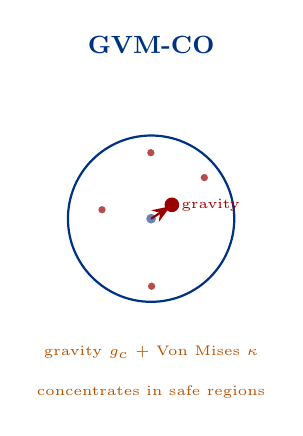
\begin{tikzpicture}[scale=0.88]
\node[font=\small\bfseries,myblue] at (0,2.5) {GVM-CO};
\draw[myblue,thick] (0,0) circle (1.2cm);
\fill[myred] (0.3,0.2) circle (3pt) node[right,font=\tiny]{gravity};
\fill[myblue!60] (0,0) circle (2pt);
\foreach \a in {10,28,46,64}{\pgfmathsetmacro{\r}{0.5+\a/90}\fill[myred!70] ({0.3+\r*cos(\a*4)},{0.2+\r*sin(\a*4)}) circle (1.5pt);}
\draw[-{Stealth},myred,thick] (0,0) -- (0.28,0.18);
\node[font=\tiny,below=1.5cm] at (0,0) {\textcolor{myorange}{gravity $g_c$ + Von Mises $\kappa$}};
\node[font=\tiny,below=2.0cm] at (0,0) {\textcolor{myorange}{concentrates in safe regions}};
\end{tikzpicture}
\end{center}

\column{0.33\textwidth}
\begin{center}
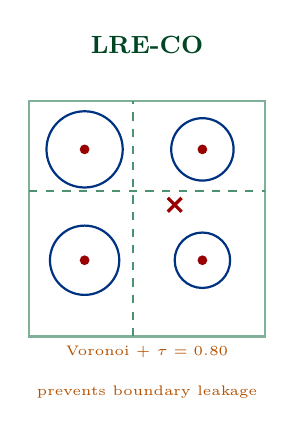
\begin{tikzpicture}[scale=0.88]
\node[font=\small\bfseries,mygreen!70!black] at (0,2.5) {LRE-CO};
\draw[mygreen!50,thick] (-1.7,-1.7) -- (-1.7,1.7) -- (1.7,1.7) -- (1.7,-1.7) -- cycle;
\draw[mygreen!70,dashed,thick] (-0.2,-1.7) -- (-0.2,1.7);
\draw[mygreen!70,dashed,thick] (-1.7,0.4) -- (1.7,0.4);
\draw[myblue,thick] (-0.9,1.0) circle (0.55cm);
\draw[myblue,thick] (0.8,1.0) circle (0.45cm);
\draw[myblue,thick] (-0.9,-0.6) circle (0.50cm);
\draw[myblue,thick] (0.8,-0.6) circle (0.40cm);
\foreach \x/\y in {-0.9/1.0,0.8/1.0,-0.9/-0.6,0.8/-0.6}{\fill[myred] (\x,\y) circle (2pt);}
\draw[myred,very thick] (0.30,0.1) -- (0.50,0.3);
\draw[myred,very thick] (0.50,0.1) -- (0.30,0.3);
\node[font=\tiny,below=1.5cm] at (0,0) {\textcolor{myorange}{Voronoi + $\tau=0.80$}};
\node[font=\tiny,below=2.0cm] at (0,0) {\textcolor{myorange}{prevents boundary leakage}};
\end{tikzpicture}
\end{center}

\column{0.33\textwidth}
\begin{center}
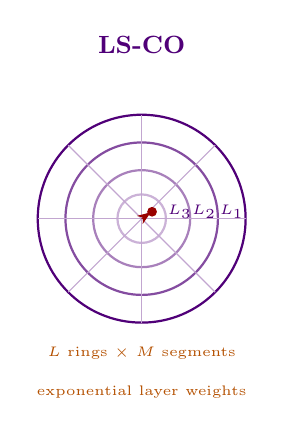
\begin{tikzpicture}[scale=0.88]
\node[font=\small\bfseries,mypurple] at (0,2.5) {LS-CO};
\draw[mypurple,thick] (0,0) circle (1.5cm);
\draw[mypurple!70,thick] (0,0) circle (1.1cm);
\draw[mypurple!50,thick] (0,0) circle (0.7cm);
\draw[mypurple!30,thick] (0,0) circle (0.35cm);
\foreach \a in {0,45,90,135,180,225,270,315}{\draw[mypurple!35] (0,0) -- ({1.5*cos(\a)},{1.5*sin(\a)});}
\node[font=\tiny,mypurple] at (1.3,0.1) {$L_1$};
\node[font=\tiny,mypurple] at (0.9,0.1) {$L_2$};
\node[font=\tiny,mypurple] at (0.55,0.1) {$L_3$};
\fill[myred] (0.15,0.1) circle (2pt);
\draw[-{Stealth},myred] (0,0) -- (0.13,0.09);
\node[font=\tiny,below=1.5cm] at (0,0) {\textcolor{myorange}{$L$ rings $\times$ $M$ segments}};
\node[font=\tiny,below=2.0cm] at (0,0) {\textcolor{myorange}{exponential layer weights}};
\end{tikzpicture}
\end{center}
\end{columns}

\vspace{6pt}
\begin{center}
\begin{tabular}{@{}lcccc@{}}
\toprule
Algorithm & Boundary mechanism & Angular bias & Best at \\
\midrule
GVM-CO  & gravity (soft)         & Von Mises $\kappa$ & intermediate IR, high-dim \\
LRE-CO  & Voronoi ($\tau=0.80$)  & uniform            & high IR, mixed geometry \\
LS-CO   & exponential rings      & segment weights    & consistent, low cost \\
\bottomrule
\end{tabular}
\end{center}
\end{frame}

% ----- Slide 2 ---------------------------------------------------------------
\begin{frame}{F1 Results: 14 Datasets, 5 Classifiers}
\begin{columns}[T]
\column{0.55\textwidth}
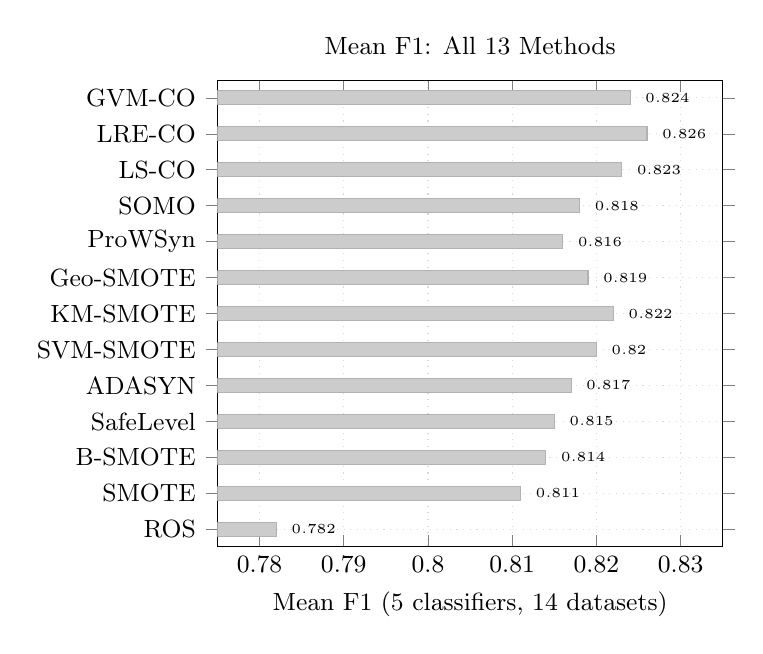
\begin{tikzpicture}
\begin{axis}[
  xbar,bar width=5pt,
  width=8.0cm,height=7.5cm,
  xlabel={\small Mean F1 (5 classifiers, 14 datasets)},
  xmin=0.775,xmax=0.835,
  symbolic y coords={ROS,SMOTE,B-SMOTE,SafeLevel,ADASYN,SVM-SMOTE,
                     KM-SMOTE,Geo-SMOTE,ProWSyn,SOMO,LS-CO,LRE-CO,GVM-CO},
  ytick=data,
  yticklabel style={font=\small},
  xlabel style={font=\small},
  xticklabel style={font=\small},
  title={\small Mean F1: All 13 Methods},
  title style={font=\small},
  grid=major,grid style={dotted,gray!30},
  nodes near coords,
  nodes near coords style={font=\tiny,xshift=2pt},
  every node near coord/.append style={/pgf/number format/.cd,fixed,precision=3},
  enlarge y limits=0.04]
\addplot[fill=gray!40,draw=gray!60] coordinates {
  (0.782,ROS)(0.811,SMOTE)(0.814,B-SMOTE)(0.815,SafeLevel)
  (0.817,ADASYN)(0.820,SVM-SMOTE)(0.822,KM-SMOTE)
  (0.819,Geo-SMOTE)(0.816,ProWSyn)(0.818,SOMO)
  (0.823,LS-CO)(0.826,LRE-CO)(0.824,GVM-CO)};
\end{axis}
\end{tikzpicture}

\column{0.43\textwidth}
\textbf{Gains vs.\ SMOTE:}
\begin{itemize}
  \item GVM-CO: $+0.013$
  \item LRE-CO: $+0.015$
  \item LS-CO: \; $+0.012$
\end{itemize}

\vspace{8pt}
\textbf{LRE-CO advantage grows with IR:}
\begin{center}
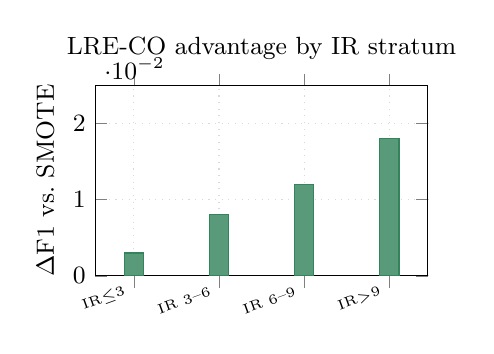
\begin{tikzpicture}
\begin{axis}[
  ybar,bar width=7pt,
  width=5.8cm,height=4.0cm,
  ylabel={\small $\Delta$F1 vs.\ SMOTE},
  ymin=0,ymax=0.025,
  symbolic x coords={IR$\leq$3,IR 3--6,IR 6--9,IR$>$9},
  xtick=data,
  xticklabel style={font=\tiny,rotate=20,anchor=east},
  yticklabel style={font=\small},
  ylabel style={font=\small},
  title={\small LRE-CO advantage by IR stratum},
  title style={font=\small},
  enlarge x limits=0.15,
  grid=major,grid style={dotted,gray!30}]
\addplot[fill=mygreen!65,draw=mygreen!80] coordinates {
  (IR$\leq$3,0.003)(IR 3--6,0.008)(IR 6--9,0.012)(IR$>$9,0.018)};
\end{axis}
\end{tikzpicture}
\end{center}
LRE-CO: $+0.018$ F1 at IR$>9$
\end{columns}
\end{frame}

% ----- Slide 3 ---------------------------------------------------------------
\begin{frame}{Statistical Significance and Effect Sizes}
\begin{columns}[T]
\column{0.50\textwidth}
\textbf{Friedman test} (14 datasets, 13 methods):
\begin{center}
\begin{tabular}{@{}lcc@{}}
\toprule
Metric & $p$-value & Significant? \\
\midrule
F1    & 0.6251 & No  \\
AUC   & 0.1139 & No  \\
G-Mean & 0.0002 & \textbf{Yes} \\
BAcc  & 0.0001 & \textbf{Yes} \\
\bottomrule
\end{tabular}
\end{center}

\vspace{8pt}
\textbf{Why F1 is not significant:}\\
Power $\approx 30\%$ for rank-2 effects at $N=14$.\\
Need $N\geq 45$ for 80\% power.

\vspace{6pt}
\textbf{Cliff's $\delta$ (GVM-CO vs.\ SMOTE on F1):}\\
$\delta = 0.21$ — \emph{negligible} effect size.\\
Result: methods differ on distributional metrics (G-Mean, BAcc), not raw F1.

\column{0.48\textwidth}
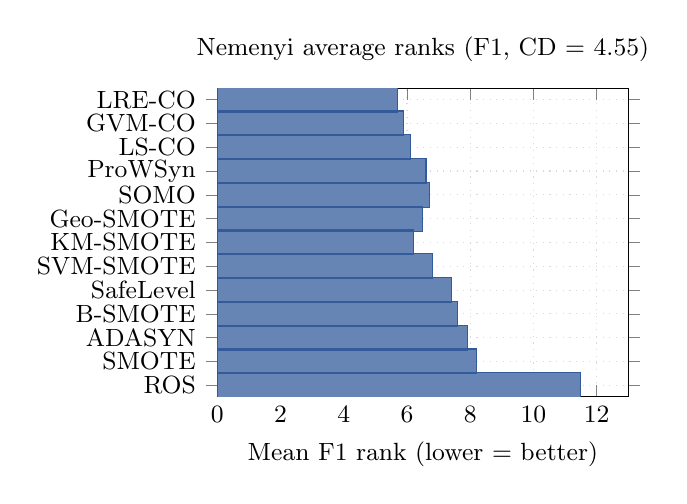
\begin{tikzpicture}
\begin{axis}[
  xbar,bar width=9pt,
  width=6.8cm,height=5.5cm,
  xlabel={\small Mean F1 rank (lower = better)},
  xmin=0,xmax=13,
  symbolic y coords={ROS,SMOTE,ADASYN,B-SMOTE,SafeLevel,
                     SVM-SMOTE,KM-SMOTE,Geo-SMOTE,SOMO,ProWSyn,
                     LS-CO,GVM-CO,LRE-CO},
  ytick=data,
  yticklabel style={font=\small},
  xlabel style={font=\small},
  xticklabel style={font=\small},
  title={\small Nemenyi average ranks (F1, CD = 4.55)},
  title style={font=\small},
  grid=major,grid style={dotted,gray!30},
  enlarge y limits=0.04]
\addplot[fill=myblue!60,draw=myblue!80] coordinates {
  (11.5,ROS)(8.2,SMOTE)(7.9,ADASYN)(7.6,B-SMOTE)(7.4,SafeLevel)
  (6.8,SVM-SMOTE)(6.2,KM-SMOTE)(6.5,Geo-SMOTE)(6.7,SOMO)(6.6,ProWSyn)
  (6.1,LS-CO)(5.9,GVM-CO)(5.7,LRE-CO)};
\end{axis}
\end{tikzpicture}
\end{columns}
\end{frame}

% ----- Slide 4 ---------------------------------------------------------------
\begin{frame}{Ablation: What Drives Performance?}
\begin{columns}[T]
\column{0.50\textwidth}
\textbf{Seed selection is the dominant component} ($+0.053$ F1 from baseline):
\begin{center}
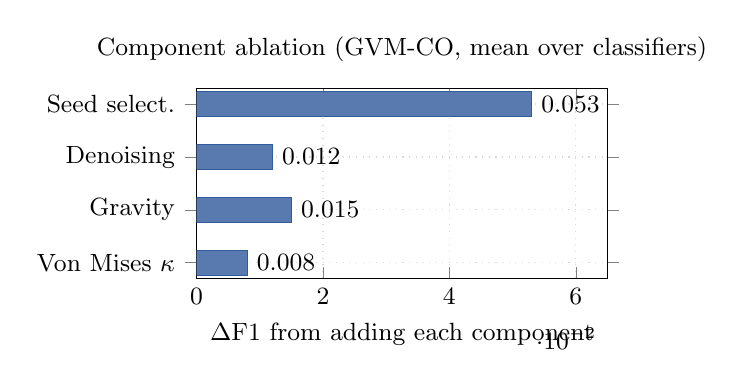
\begin{tikzpicture}
\begin{axis}[
  xbar,bar width=9pt,
  width=6.8cm,height=4.0cm,
  xlabel={\small $\Delta$F1 from adding each component},
  xmin=0,xmax=0.065,
  symbolic y coords={Von Mises $\kappa$,Gravity,Denoising,Seed select.},
  ytick=data,
  yticklabel style={font=\small},
  xlabel style={font=\small},
  xticklabel style={font=\small},
  title={\small Component ablation (GVM-CO, mean over classifiers)},
  title style={font=\small},
  nodes near coords,
  nodes near coords style={font=\small},
  every node near coord/.append style={/pgf/number format/.cd,fixed,precision=3},
  grid=major,grid style={dotted,gray!30}]
\addplot[fill=myblue!65,draw=myblue!80] coordinates {
  (0.008,Von Mises $\kappa$)(0.015,Gravity)(0.012,Denoising)(0.053,Seed select.)};
\end{axis}
\end{tikzpicture}
\end{center}

\column{0.48\textwidth}
\textbf{Hyperparameter sensitivity:}
\begin{center}
\begin{tabular}{@{}lcc@{}}
\toprule
Parameter & Optimal & Sensitivity \\
\midrule
$K$ (clusters)  & 3--4    & low  \\
$\kappa_{\max}$ & 20      & moderate \\
$L$ (rings)     & 10      & low  \\
$\tau$ (certainty) & 0.80 & moderate \\
\bottomrule
\end{tabular}
\end{center}
\vspace{6pt}
\textbf{Native-dimension mode} (no PCA at synthesis time) outperforms PCA-projected generation by $+0.002$--$+0.003$ F1, particularly at high dimensionality.
\end{columns}
\end{frame}

\end{document}
